\section{Gráficos y análisis}
Para probar la herramienta desarrollada en la primera parte, se analizaron cuatro redes diferentes a partir de las dos fuentes de información, el Modelo Ethernet y el Modelo ARP. 
A continuación se presentan las cuatro LANs analizadas y sus correspondientes resultados. 

\subsection{Digrafos de las redes}\label{"Grafos"}

\subsubsection{Red Hogareña}
Como lo indica su nombre, la misma fue tomada en la casa de uno de los integrantes del grupo. Utilizandose la red Wifi se realizaron capturas de los paquetes Ethernet y, además, de los ARP, de acuerdo al modelo correspondiente. La red presentaba pocos dispositivos conectados y enviando y recibiendo información, por lo que permite un mejor análisis del comportamiento de la misma. 

A continuación se presenta un digrafo que muestra el comportamiento de la red para el Modelo ARP. Se presentan en los nodos a los dispositivos con su correspondiente dirección IP y las aristas corresponden a la cantidad de paquetes de tipo Replay o Request que ocurren entre dos host. 

\begin{figure}{h!}{0.5\textwidth}
  \begin{center}
    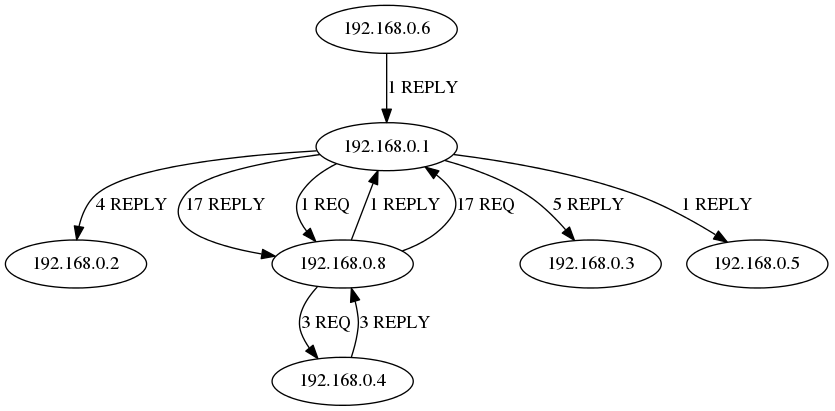
\includegraphics[width=1\textwidth]{./graficos/grafos-arp/grafo_casa_mari.png}
  \end{center}
  \caption{Digrafo: red hogareña}
\end{figure}

Como se puede observar, el host con dirección IP 192.168.0.1 se podría inferir que es el router, ya que es el capaz de responder con un mensaje de tipo Replay a todos los mensajes de tipo Request enviados. Luego, en secciones siguientes se podrá distinguir de manera clara cual representaría al nodo distinguido para el evento del Modelo ARP. 

\subsubsection{Red Laboratorio}
En este caso se decidió capturar los paquetes que se encontraban en la red cableada de uno de los laboratorios de la facultad. La cantidad de host que se encuentran interviniendo en la misma es mucho mayor a la de una red hogareña. Se muestra, a continuación, el digrafo generado a partir del evento ``una dirección IP participa en el envío de un paquete de tipo Replay o Request a otra dirección IP''. 

Debido al gran número de dispositivos que se involucran en la red, se decidió eliminar aquellos que únicamente participan en el recibimiento o envío de un solo paquete de tipo ARP. Ese filtro se aplica únicamente para la presentación del digrafo del evento ``una dirección IP participa en el envío de un paquete de tipo Replay o Request a otra dirección IP''.

\begin{figure}{h!}{0.5\textwidth}
  \begin{center}
    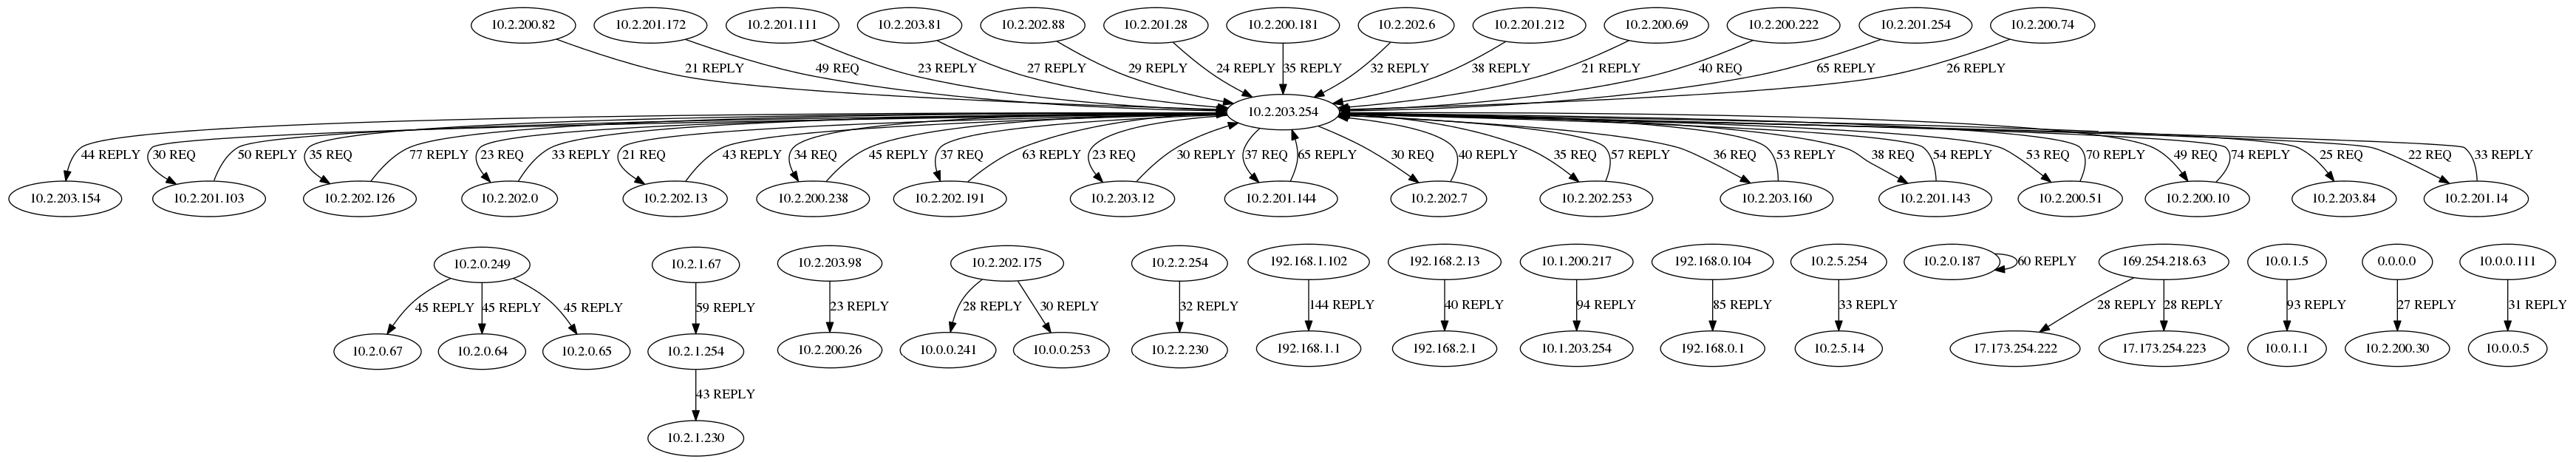
\includegraphics[angle=90, scale=0.3]{./graficos/grafos-arp/grafo_labo5.png}
  \end{center}
  \caption{Digrafo: red laboratorio}
\end{figure}

A partir del digrafo, se podría concluir que el nodo 10.2.203.254 es un nodo característico debido a la cantidad de información que posee. Luego, mediante otro tipo de análisis, se podrá definir de manera más clara, cual es el nodo característico correspondiente a esa fuente de información para la Red del Laboratorio. 


\subsubsection{Red Devartis}
Otra de las capturas se realizó en el trabajo de uno de los integrantes. Los paquetes se capturaron en la red cableada del lugar. Esta red cuenta con aproximadamente 16 host, 1 router y 1 servidor. Es decir, la red presenta un tamaño intermedio con respecto a las dos anteriores. Por lo que es más compleja de analizar que la red hogareña, pero mucho más simple que la red del laboratorio de la facultad. 
Debajo, se puede observar el digrafo obtenido. El mismo fue originado a partir del mismo evento que los anteriores. 

\begin{figure}{h!}{0.5\textwidth}
  \begin{center}
    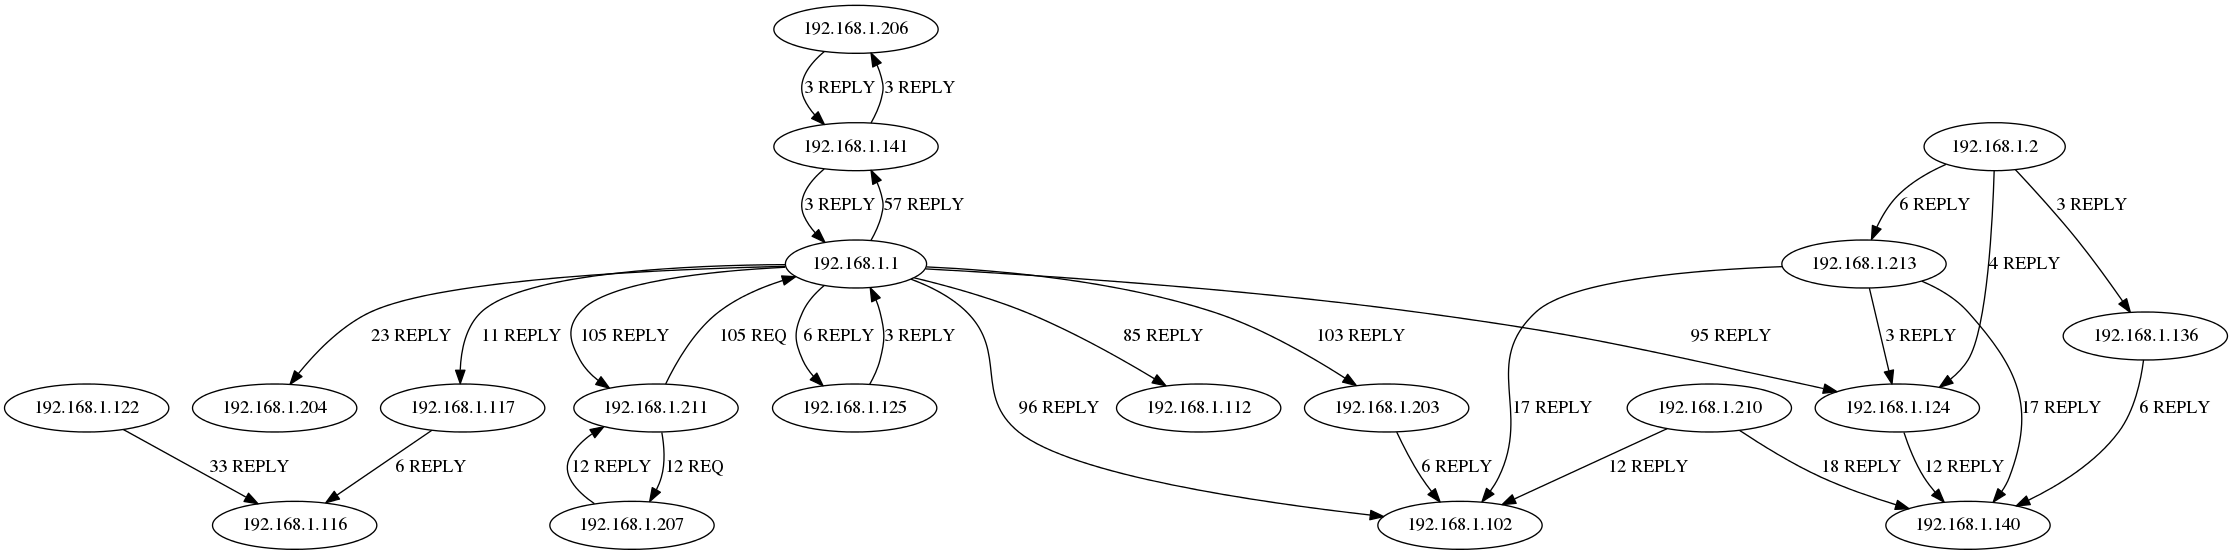
\includegraphics[angle=90, scale=0.3]{./graficos/grafos-arp/grafo_laburo_mari.png}
  \end{center}
  \caption{Digrafo: red laboral Devartis}
\end{figure}

Observando el grafo presentado, se puede notar que el nodo 192.168.1.1 es distinguido, por la cantidad de mensajes de tipo Replay que salen de mismo. Probablemente, la IP del nodo corresponda al router de la red. Esta  deducción, se podrá comprobar en el análisis de siguientes gráficos.

\subsubsection{Red Mercap}
Finalmente, la cuarta captura se realizó en el trabajo de otro de los integrantes. La red fue analizada desde una máquina virtual corriendo un sistema Linux, sobre un host Windows. Cabe aclarar que la misma estaba conectada a la red de manera física y que cuenta de 30 computadoras, 5 servidores y 1 router WiFi (además de los posibles dispositivos móviles conectados a la red de manera inalámbrica).

La captura duró una hora, durante la cual se obtuvo una enorme cantidad de relaciones generadas entre los diferentes actores, enviando y recibiendo los respectivos paquetes ARP. Esto ya aseguraba que el digrafo resultante (en primer instancia) iba a ser ilegible, aún ampliando la imagen (como observamos en el círculo con zoom sobre uno de los tantos nodos distinguidos de la red). 

Es por eso que para analizar mejor la red y la interacción por medio de paquetes, decidimos mostrar solo aquellas relaciones en las cuales se envíen o reciban mas de 20 paquetes ARP. Este filtro solo se aplica para favorecer la visualización de los datos y de ninguna manera alteramos los resultados de la captura para los experimentos posteriores. De esta manera, observamos que la presente red toma un tamaño mucho mas manejable. Limitando la cantidad de nodos a mostrar, nos podemos concentrar en ver los nodos que realmente se destacan.

A simple vista observamos que los nodos 192.168.168.1, 192.168.168.2, 192.168.168.4, 192.168.168.36 y 192.168.168.135 concentran gran parte del intercambio de mensajes ARP de este segmento de la captura. De estos nodos distinguidos, en particular podemos inferir que los que tienen IPs mas bajas, probablemente sean algunos de los servidores de los que dispone la empresa. Potencialmente, los mas antiguos y utilizados, a saber; un servidor para Envy (control de versiones orientado a objetos - Smalltalk), un servidor que aloja la web empresarial, un CVS y otras herramientas como JIRA ó BambooHR (muy consultados a toda hora), y finalmente un servidor corriendo GemStone (base de datos no relacional).

\begin{figure}{h!}{0.5\textwidth}
  \begin{center}
    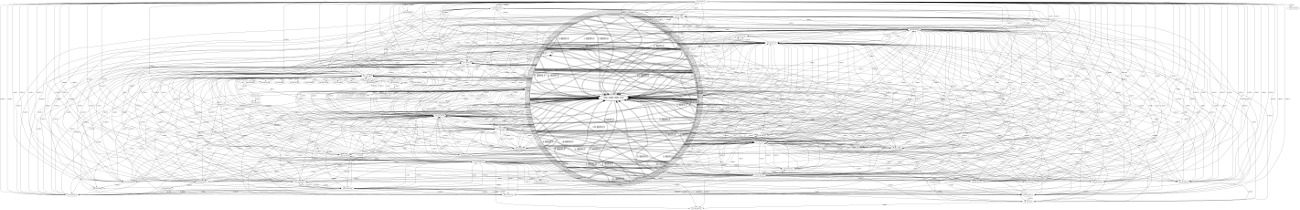
\includegraphics[angle=90,scale=0.2]{./graficos/grafos-arp/grafo_laburo_eze1.png}
  \end{center}
  \caption{Digrafo: red laboral Mercap}
\end{figure}